\documentclass{beamer}
\usetheme{Madrid}
\usecolortheme{default}

\title[Social Connections Analysis]
{Effects of Socialization on Mental Health}

\subtitle{STA130 Course Project}

\author[STA130] % (optional, for multiple authors)
{Edie Chen \and Jason Li \and Zain Mahmoud \and Rana Nagash\\
TA Oliver Gatalo\\
Professor Scott Schwartz}

\institute[UofT] % (optional)
{
  STA130: An Introduction to Statistical Reasoning and Data Science\\
  Department of Statistical Sciences\\
  University of Toronto
}

\date[November 2024] % (optional)


\logo{
\includegraphics[height=0.8cm]{logo_uoft}}

\definecolor{uoftblue}{RGB}{6,41,88}
\setbeamercolor{titlelike}{bg=uoftblue}
\setbeamerfont{title}{series=\bfseries}

\begin{document}

\frame{\titlepage}


\section{Introduction}

\begin{frame}
\frametitle{Introduction}
Social interactions play a pivotal role in shaping individual mental health outcomes. It is becoming increasingly easier, especially for teenagers, to connect with their friends virtually from the comfort of their homes. One may argue that this is harmful for their mental health; is this always the case?\\
Through this research, we aim to highlight the difference between physically interacting with community members as opposed to virtually connecting with them. We used the \alert{Canadian Social Connections Survey (CSCS)} to investigate the relationship between various forms of social interactions (physical and non-physical) and how they affect the individuals' mental health states. 
This presentation outlines the variables we're using, our hypotheses, analyses, key findings, and the conclusions we've drawn from these findings.
\end{frame}


\section{Research questions}

\begin{frame}
\frametitle{Our research questions}

\begin{block}{Question 1}
    Is there an association between the frequency of days where an individual spends at least 5 minutes physically socializing and their level of depression?
\end{block}

\begin{block}{Question 2}
Is there an association between playing video games and feeling depressed, and can going on walks counteract that?
\end{block}

\begin{block}{Question 3}
    How does the association between loneliness and video chatting compare to text messaging?
\end{block}
\end{frame}
\section{Question 1}
\begin{frame}
\frametitle{Question 1: Variables}

Independent variables:

\vspace{1em}

{\small{\tt CONNECTION\_social\_days\_family\_p7d\_grouped}:\\
days where individuals spent at least 5 minutes socializing with family.}

\vspace{0.5em}

{\small{\tt CONNECTION\_social\_days\_friends\_p7d\_grouped}:\\
days where individuals spent at least 5 minutes socializing with friends.}

\vspace{0.5em}

{\small{\tt CONNECTION\_social\_days\_coworkers\_and\_classmates\_p7d\_grouped}:\\
days where individuals spent at least 5 minutes socializing with co-workers or classmates.}

\vspace{0.5em}

{\small{\tt CONNECTION\_social\_days\_neighbours\_p7d\_grouped}:\\
days where individuals spent at least 5 minutes socializing with neighbours.}

\vspace{1.5em}

Dependent variable:

{\small{\tt WELLNESS\_phq\_score}:\\
metric used to characterize an individual's level of depression on a scale\\
of 0-6.}


\end{frame}


\begin{frame}{Preliminary analysis}

    The independent variables were categorical with 4 categories each: 
\begin{figure}
    \centering
    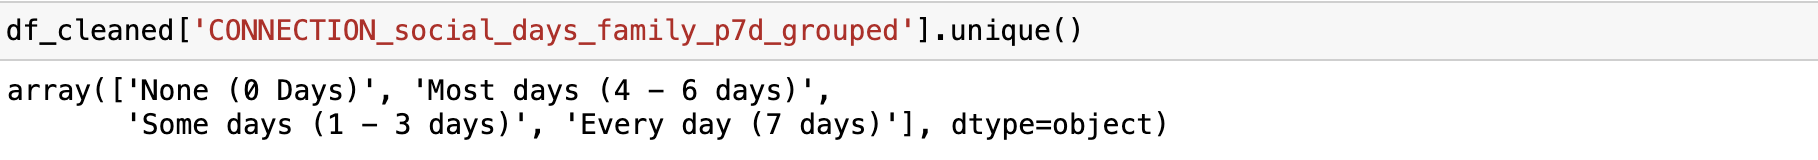
\includegraphics[width=1\linewidth]{image2.png}
    \caption{Unique data entries in one of the columns }
    \end{figure}
    To better analyze the data, we gave each category a numeric value based on the midpoint of the interval. For example, the 'Most days (4-6)' category was assigned 5 (representing the midpoint of the number of days). Then, we added another column to represent the total number of days where each individual spent at least 5 minutes socializing with any one of the groups above using the numeric values we assigned to each category. 
\end{frame}


\begin{frame}{Analysis}
    First, we examined the relationship between the total column and the numeric PHQ score column. We did this by fitting a simple linear regression through the data.
    \begin{columns}
        \column{0.5\textwidth}
        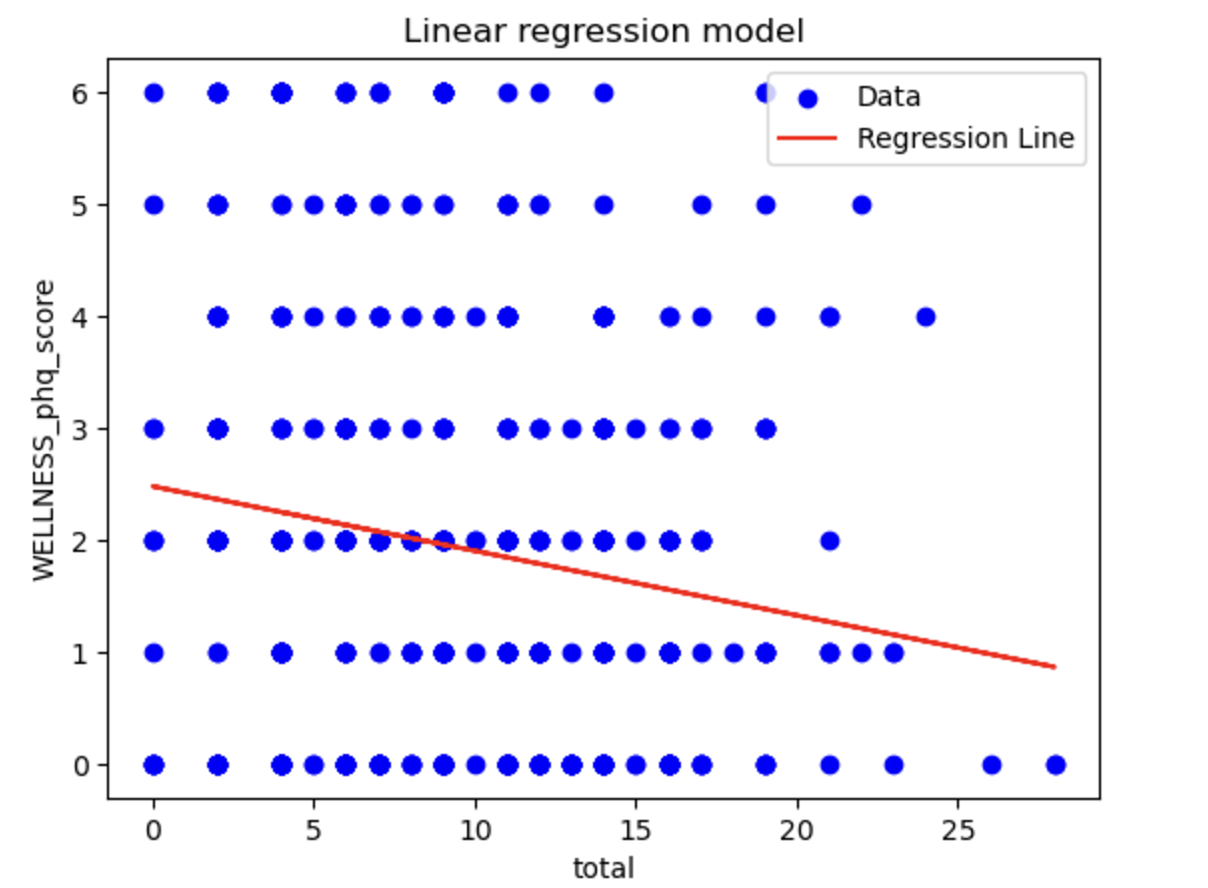
\includegraphics[width=1\linewidth]{model1.png}\\
        \column{0.5\textwidth}
        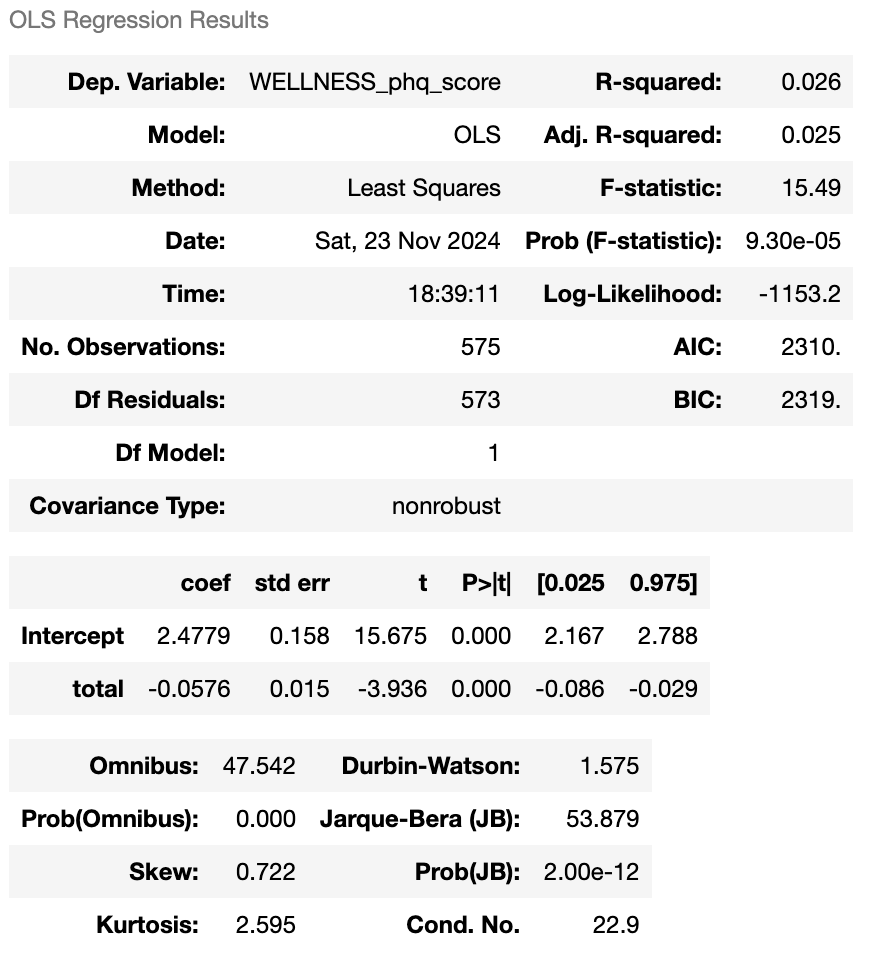
\includegraphics[width=1\linewidth]{summarystats.png}

        
    \end{columns}
\end{frame}

\begin{frame}{Limitations and assumptions}

    For this analysis, we only considered days where individuals spent at least 5 minutes socializing. However, this threshold is vague and is not specific enough. One could spend 5 minutes socializing and another could spend 5 hours socializing yet they would still be considered under the same category. I also made some assumptions to convert the categorical values into numeric values. However, given that the mapping of involved the midpoint of each interval, I believe this conversion was suitable.
    
\end{frame}

\begin{frame}{Analysis}
    We then created a bootstrapped distribution of model slope coefficients by repeatedly resampling from our original sample and refitting OLS models through the samples. Then, we created a 95\% confidence interval of our bootstrapped coefficients for inference.
    \begin{figure}
        \centering
        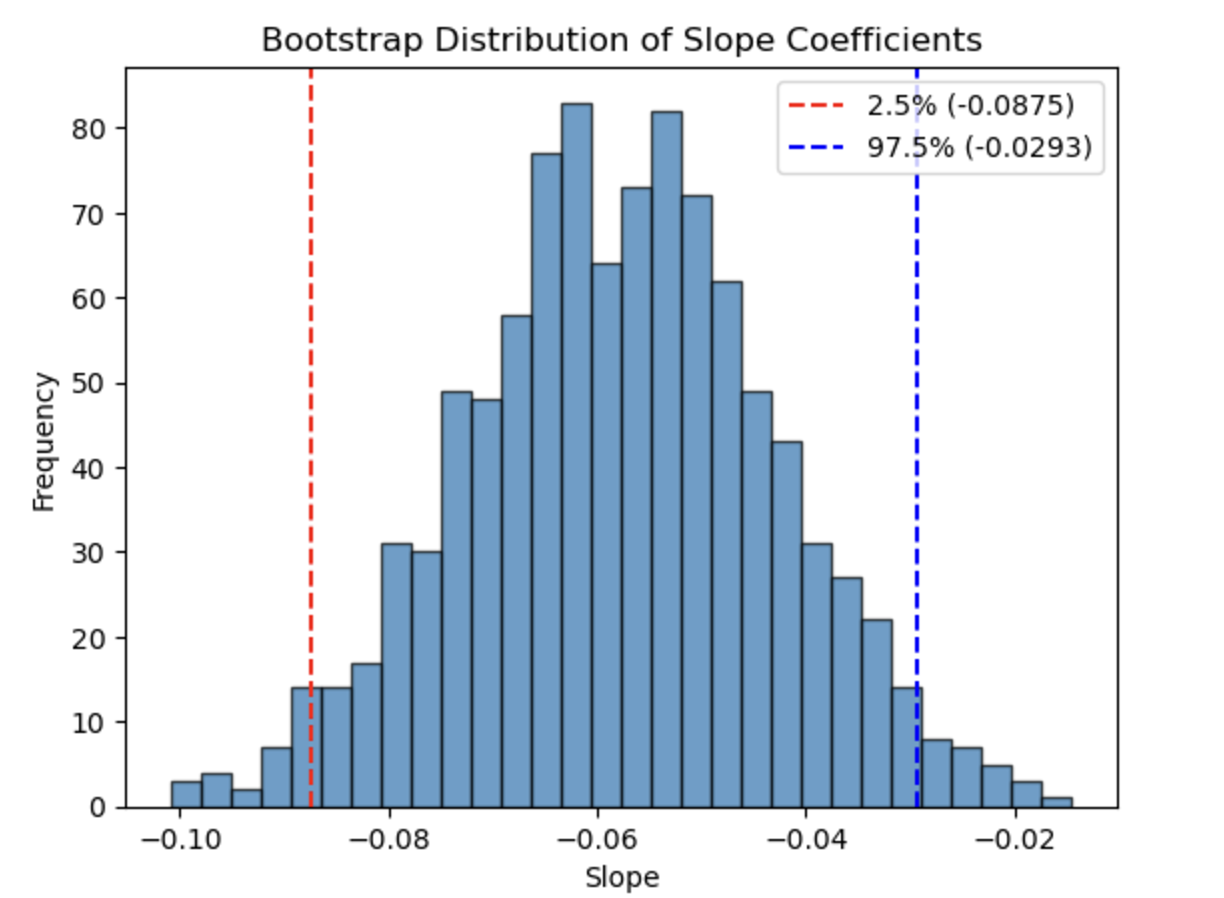
\includegraphics[width=0.5\linewidth]{95CI.png}
        \caption{95\% confidence interval}
        \label{fig:enter-label}
    \end{figure}
\end{frame}

\begin{frame}{Summary and conclusion}
The confidence interval we constructed only contained negative slopes between $-0.0875$ and $-0.0293$ and so we can conclude with 95\% confidence that the true value of the slope coefficient lies in that interval. This means that as the number of days where an individual spends at least 5 minutes socializing increases, the average depression score decreases. However, the values of the slopes are very small and so the effect of socializing on depression scores is minuscule.
    
\end{frame}






% Jason

\section{Question 2}

\begin{frame}
    \frametitle{Question 2: Variables}
    
    Independent variables:
    
    \vspace{1em}
    
    {\small{\tt CONNECTION\_activities\_onlinegames\_p3m}:\\
    how often an individual has played online games in the past 3 months}\\
    {\tiny \textbf{Ordinal categorical outcomes:} Not in the past three months, Less than monthly, Monthly, A few times a month, Weekly, A few times a week, Daily or almost daily}

    
    \vspace{0.5em}
    
    {\small{\tt CONNECTION\_activities\_walk\_p3m}:\\
    how often an individual has gone on a walk with friends in the past 3 months}\\
    {\tiny \textbf{Ordinal categorical outcomes:} Not in the past three months, Less than monthly, Monthly, A few times a month, Weekly, A few times a week, Daily or almost daily}
    
    \vspace{1.5em}
    
    Dependent variable:

    \vspace{1em}
    
    {\small{\tt WELLNESS\_malach\_pines\_burnout\_measure\_depressed}:\\
    how often an individual feels depressed}
    {\tiny \textbf{Ordinal categorical outcomes:} Never, Almost never, Rarely, Sometimes, Very Often, Always}
    
    
\end{frame}

\begin{frame}
    \frametitle{Limitations and assumptions}

    It is not possible to perfectly map the ordinal categories for how often an individual feels depressed {\tiny Never, Almost never, Rarely, Sometimes, Very Often, Always} numerically.

    It shouldn't be assumed that the "distance" between each category is "1", but I will map it to the numbers 0 through 5 for multiple linear regression.

    \vspace{1em}

    It is not possible to measure level of depression in a binary variable, if I wanted to do something like a logistic regression.

    \vspace{1em}

    I will keep the outcomes as a continuous variable (intended to be interpreted from a 0 through 5 scale), rather than converting it back to categorical.

\end{frame}


\begin{frame}
    \frametitle{Cleaning data}

    First, I want to assign numbers to the ordinal categories of how often an individual feels depressed.

    I will just use the consecutive numbers 0 (never) through 5 (always).

    \begin{figure}
        \centering
        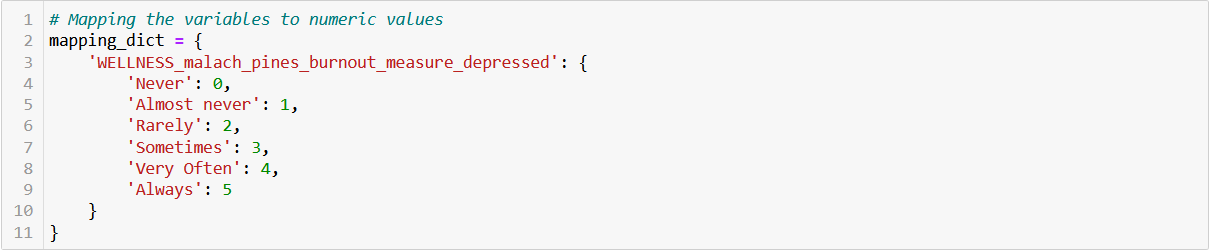
\includegraphics[width=0.8\linewidth]{jason_depressionvalues.png}
    \end{figure}

    After renaming variables, removing empty values, etc., this is what my DataFrame looks like.

    \begin{figure}
        \centering
        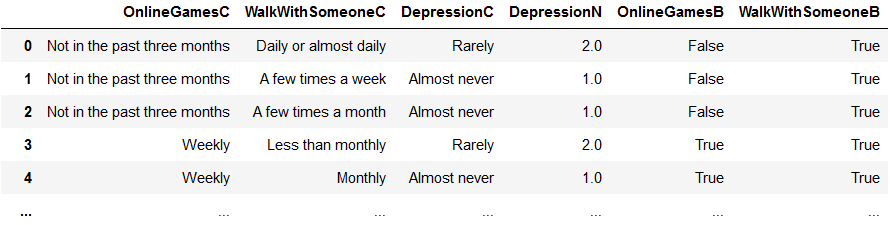
\includegraphics[width=0.5\linewidth]{jason_dfpreview.png}
    \end{figure}
    
\end{frame}


\begin{frame}

    \frametitle{Multiple Linear Regression}
    
    The table below retains only the significant (p-value $\leq 0.05$) outcomes (rest are omitted) from a multiple linear regression.
    I will create a new column that will show the predicted $\hat y$ values, and plot this on a bar plot.
    \begin{figure}
        \centering
        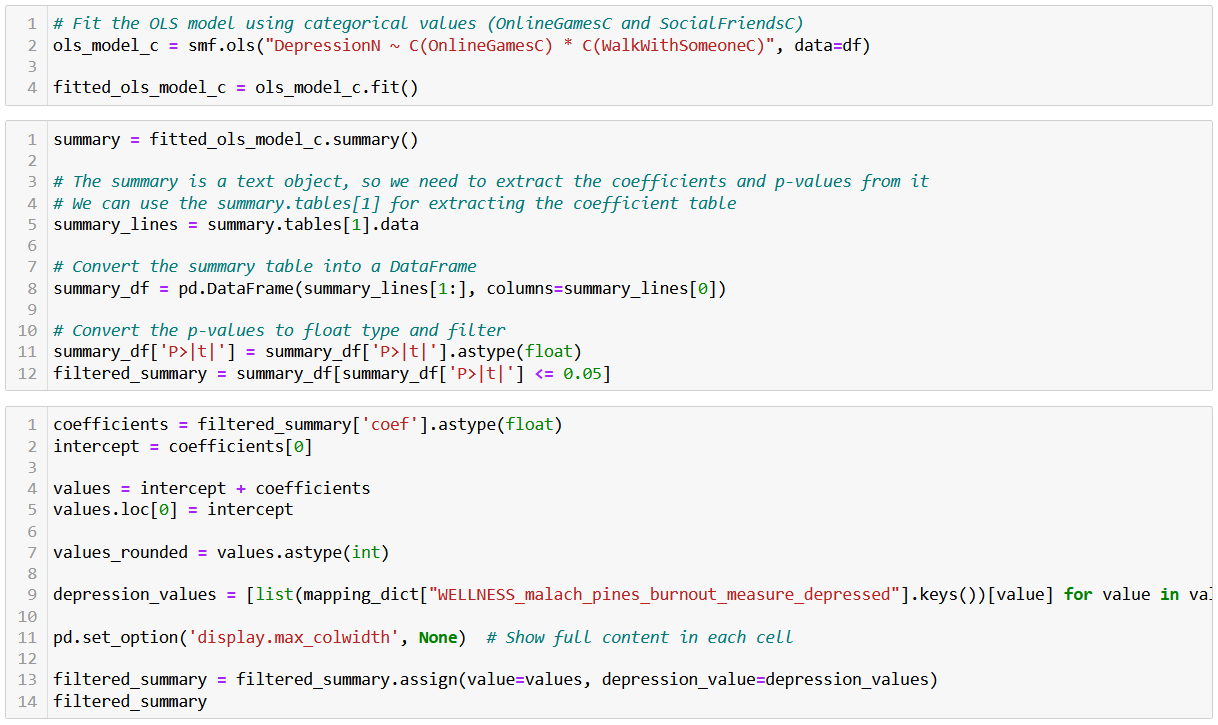
\includegraphics[width=0.3\linewidth]{jason_regression.png}
        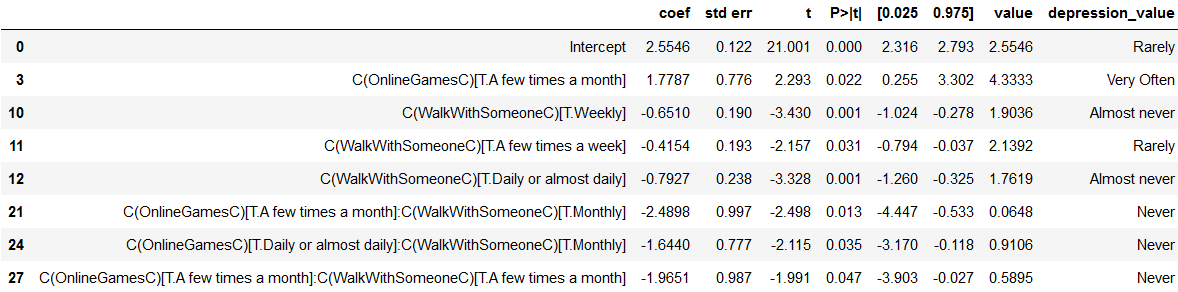
\includegraphics[width=0.8\linewidth]{jason_regressionoutcome.png}
    \end{figure}
    
    \end{frame}

\begin{frame}
    \frametitle{Bar plot}

    {\tiny Sorted in descending order, with intercept first.}

    \begin{figure}
        \centering
        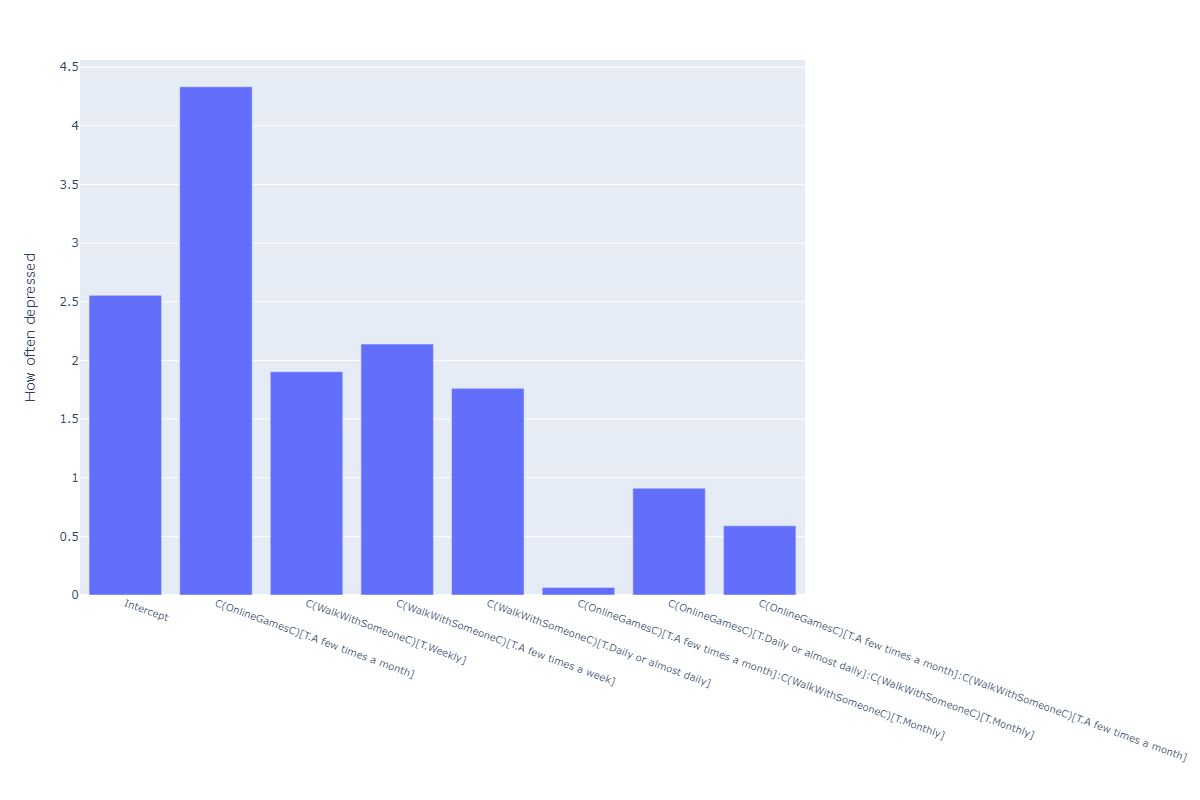
\includegraphics[width=1\linewidth]{jason_barplot.png}
    \end{figure}

\end{frame}


\begin{frame}
    \frametitle{Findings}

    Recall that the values on the bar chart is how level of depression changes as the variables in the x-axis changes.

    We find that the intercept (no online games, no going on walks with friends) is 2.5 on this 0-5 scale. It is interesting that the intercept is at the halfway point.
    
    We find that even just playing online games a few times a month can increase one's level of depression a lot.

    As an individual's frequency on walks with friends increases, their level of depression decreases.

    This change is apparant in playing and not playing online games.

    In conclusion, we find that only playing online games will correlates positively with one's level of depression, while going on walks with friends will significantly lower that.

\end{frame}






\section{Question 3}
%ADD YOUR FRAMES BELOW
\begin{frame}{Question 3 Variables}

\small % Makes the text smaller
How does the association between loneliness and video chatting compare
to text messaging?\\

\vspace{0.5em} % Adds space between lines
\textbf{Independent Variables:}\\
\vspace{0.2em}
Video chatted with friends/family in the past 3 months:\\
Texted or messaged someone in the past 3 months to check in:\\

\vspace{0.5em}
7 Options:
\begin{itemize}
    "Not in the past three months" ...
    "Daily or almost daily",
\end{itemize}

\vspace{0.5em}
\textbf{Dependent Variables:}\\
\vspace{0.2em}
How many days felt lonely in the past week:\\

\vspace{0.5em}
5 Options:
\begin{itemize}
    'None of the time (e.g., 0 days)': 0 ... 'All of the time (e.g. 5-7 days)': 6
\end{itemize}

\end{frame}

\begin{frame}
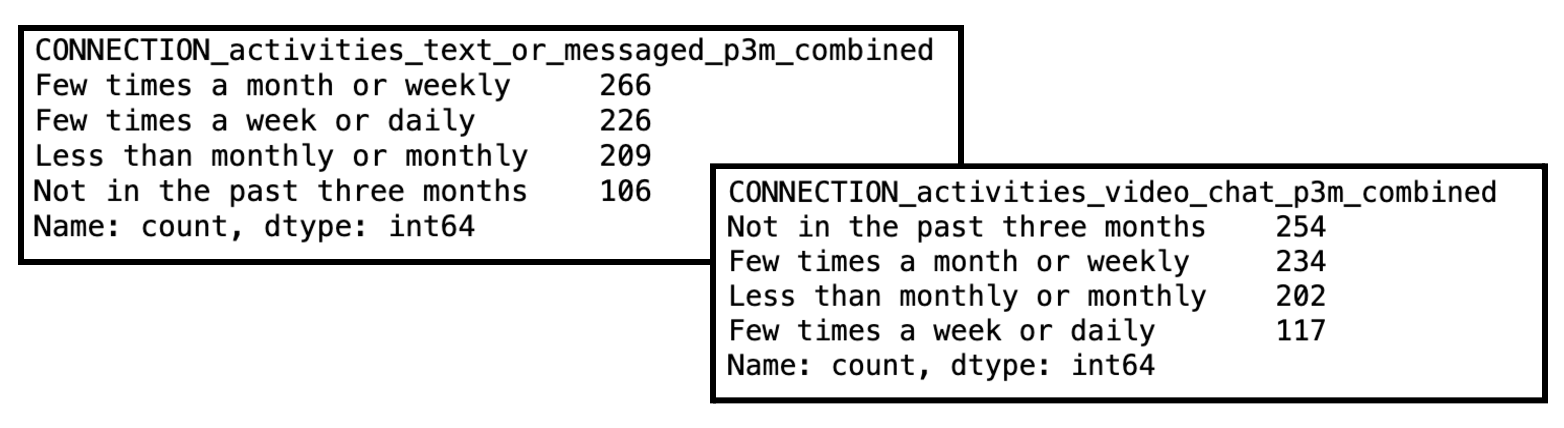
\includegraphics[width=\linewidth]{Screenshot 2024-12-01 at 12.16.24 PM.png}
We combined the independent variables into categories of two options to reduce the number of options from 7 to 4\\
More narrowed down results\\
\vspace{1em}
\small We selected "Few times a month or weekly" as the baseline (since it is a moderate level of frequency)
\end{frame}

\begin{frame}{Assumptions}
\begin{itemize}
    \item Converting the categorical variable to numerical values makes it not completely accurate since it assumes an exact number of days that they feel lonely (it is not a continuous variable but it being treated as one)\\
    \item How many days people feel lonely in a week is not reflective of how lonely they feel on average\\
    \item Converting independent variables into 4 categories of options instead of 7 is not reflective of how the surveyors actually responded to the question and narrows down the frequency of their activities
\end{itemize}
\end{frame}

\begin{frame}{Visualization of the Raw Data}

\begin{minipage}[t]{0.51\linewidth} % Reduced width
    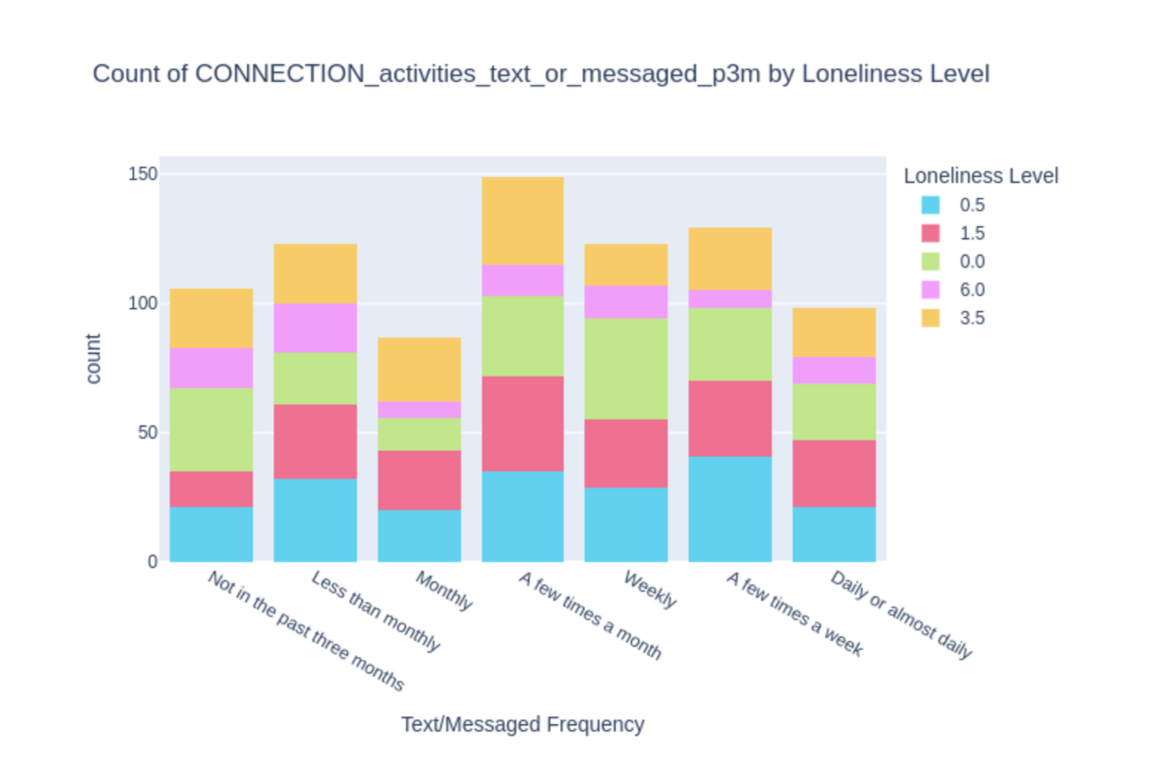
\includegraphics[width=\linewidth]{Screenshot 2024-11-28 at 12.28.29 PM.png}
    \caption{Graph 1 - Text/Messaged} % Optional caption
\end{minipage}%
\hspace{-1em} % Reduces space between the minipages
\begin{minipage}[t]{0.51\linewidth} % Same width as the first minipage
    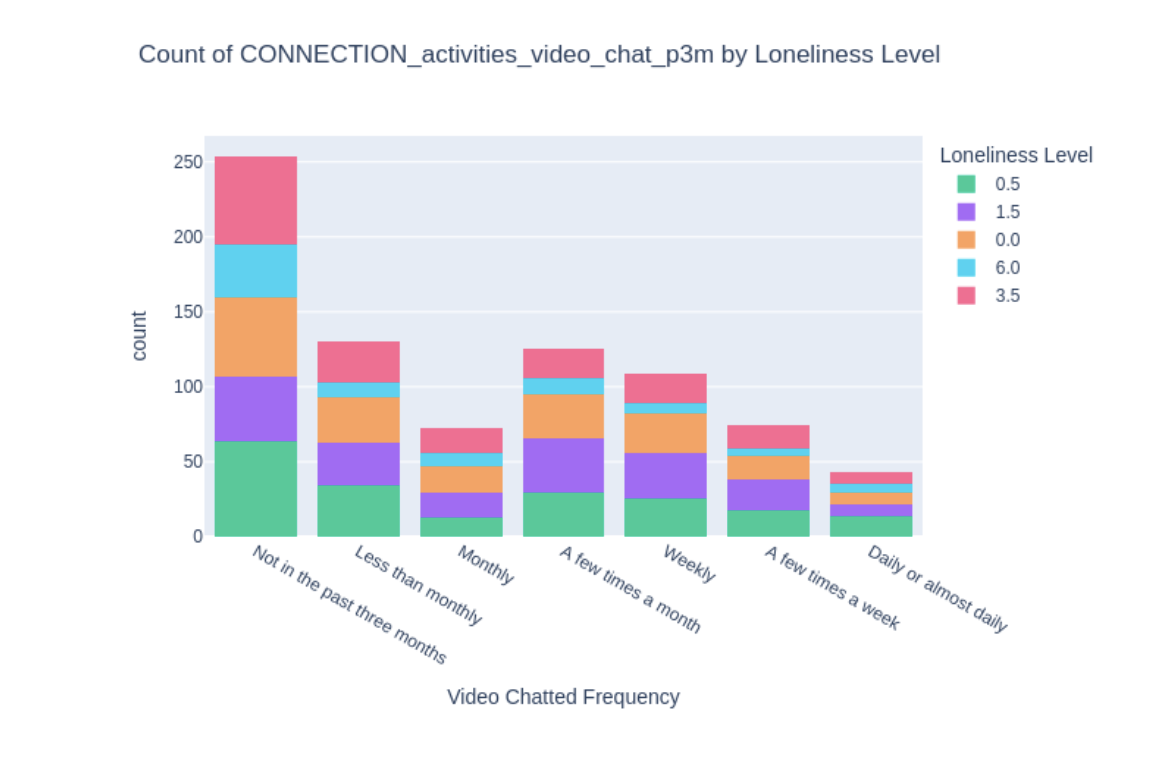
\includegraphics[width=\linewidth]{Screenshot 2024-11-28 at 12.31.04 PM.png}
    \caption{Graph 2 - Video Chatting} % Optional caption
\end{minipage}

\end{frame}


\begin{frame}{ Simple Linear Regression \& Data Wrangling} % Tiny text in title too

\small % Reduces text size for the entire frame
We first tried to analyze the two factors separately with simple linear regression.\\

\vspace{0.5em} % Adds space before the images

\begin{minipage}[t]{0.49\linewidth}
    \centering
    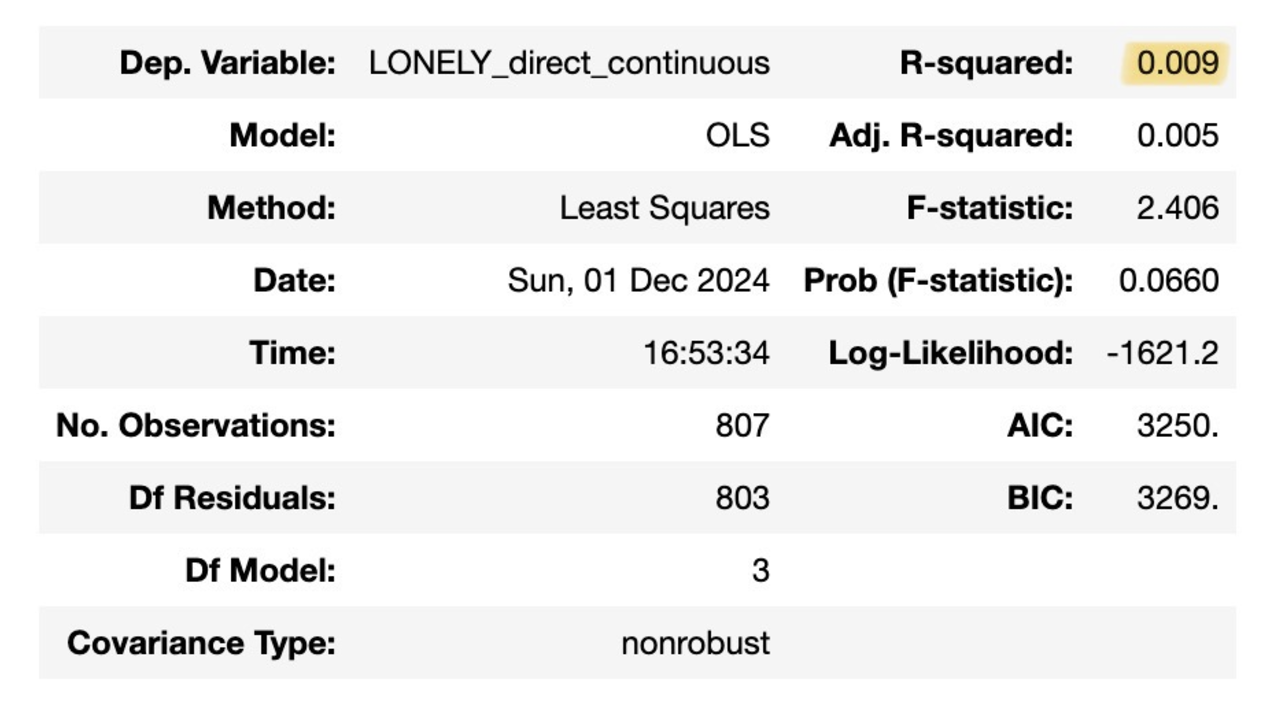
\includegraphics[width=\linewidth]{Screenshot 2024-12-01 at 12.01.04 PM.png}\\
    Loneliness vs. Video Chatting Frequency
\end{minipage}%
\hfill%
\begin{minipage}[t]{0.49\linewidth}
    \centering
    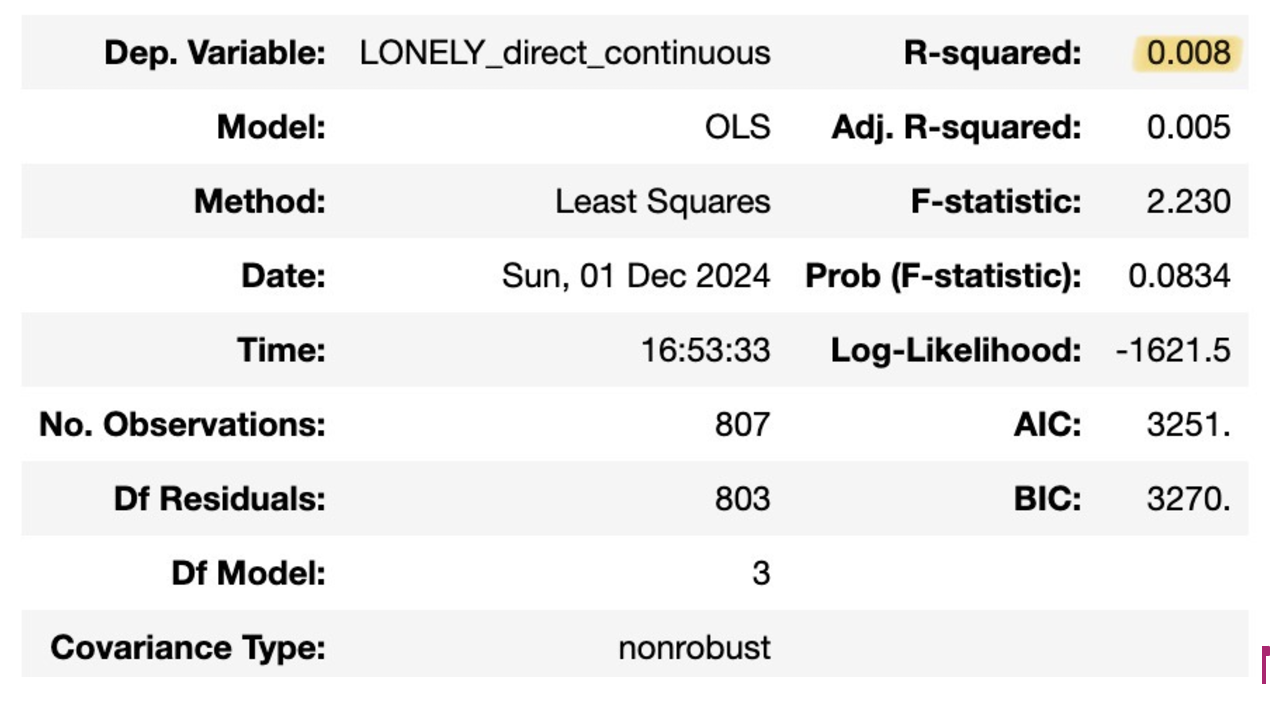
\includegraphics[width=\linewidth]{Screenshot 2024-12-01 at 12.01.09 PM.png}\\
    Loneliness vs. Text Messaging Frequency
\end{minipage}

\vspace{0.5em} % Adds space after the images

The fitting of the model was poor, so we decided to analyze with a multilinear regression model with interactions.\\

\end{frame}


\begin{frame}{Final Result \& Analysis}

\begin{minipage}[t]{0.6\linewidth} % Adjust width for the image
    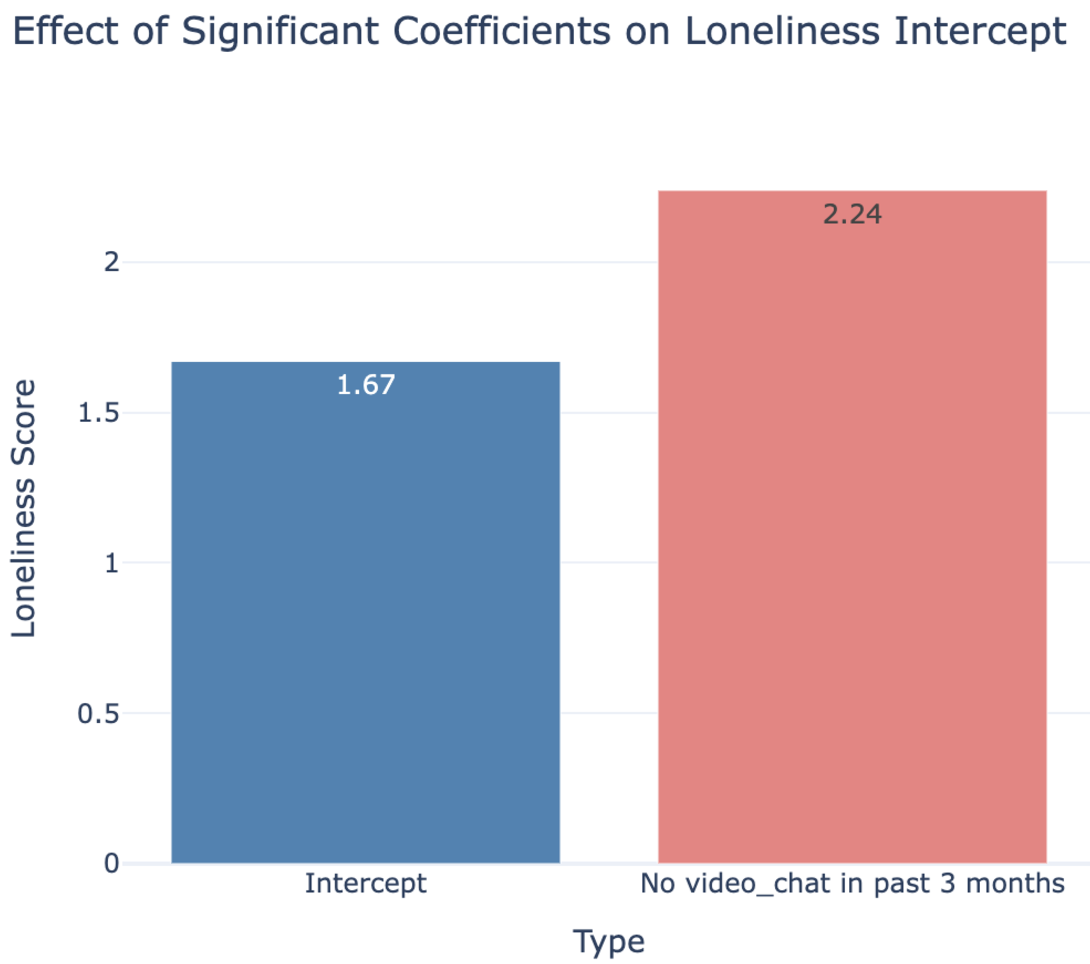
\includegraphics[width=\linewidth]{Screenshot 2024-12-01 at 1.08.25 PM.png}
\end{minipage}%
R-squared value = 0.32\\
The condition number = 26.4\\
Residual analysis suggests minimal bias\\

\end{frame}

\begin{frame}
\textbf{Conclusions:}\\
\begin{itemize}
    \item  Treating texting and video chatting a few times a month or weekly as the baseline
    \item Comparing that intercept to no video chat in the past 3 months
    \item Final Result - Not video chatting in the past 3 months increases the days one feels lonely from 1.67 (when texting and video chatting a few times a month or weekly) to 2.24 days\\
    \item So, video chatting could be beneficial to reducing loneliness 
\end{itemize}

*Reminder that this is not completely accurate due to assumptions mentioned previously\\
*Reminder that correlation $\neq$ causation
\end{frame}

\section{Question 3}
%ADD YOUR FRAMES BELOW

\begin{frame}{Conclusion}

\textbf{Connections}\\
\begin{itemize}
    \item Aim to analyze how people’s mental health is associated with different socializing forms
\end{itemize}

\textbf{Findings}\\ 
\begin{itemize}
    \item Socializing and Depression:
    \begin{itemize}
        \item The average depression score decreases when physical socialization $\geq $ 5 min/day
        \item Depression levels also drop when taking a walk with others.
        \item Playing video games, however, may have an opposing effect on depression levels.
    \end{itemize}
    \item Socializing and Loneliness:
    \begin{itemize}
        \item Not video chatting in the past 3 months increases the days one feels lonely
    \end{itemize}
\end{itemize}
    
\end{frame}

\end{document}